\message{ !name(sumarioExecutivo.tex)}
\documentclass[10pt,a4paper]{article}
\usepackage{ifpdf}
\usepackage[utf8]{inputenc}
\usepackage[portuges]{babel}
\usepackage{float}
\usepackage{graphicx}
\usepackage{enumerate}
\usepackage{url}
\usepackage[top=2cm,left=2cm,right=2cm,bottom=2cm]{geometry}
\title{Analise de metodos de seleção para algoritmos genéticos}
\author{Anderson Gonçalves Marco}
\usepackage{amsmath}
\usepackage{array}
\newcolumntype{L}[1]{>{\raggedright\let\newline\\\arraybackslash\hspace{0pt}}m{#1}}
\newcolumntype{C}[1]{>{\centering\let\newline\\\arraybackslash\hspace{0pt}}m{#1}}
\newcolumntype{R}[1]{>{\raggedleft\let\newline\\\arraybackslash\hspace{0pt}}m{#1}}
{\renewcommand{\arraystretch}{1.4}%

\begin{document}

\message{ !name(sumarioExecutivo.tex) !offset(-3) }

\maketitle
\section{Introdução}
Problemas de otmização são importantes em diferentes areas da ciencia como a engenharia de produção, mecanica e logistica. Nestes tipos de problemas tenta-se conceseguir o maximo de resultado com o minimo de recursos. Os algoritmos geneticos são extremamentes importantes para  resolução destes problemas, eles são metodos baseados na teoria de evolução de Charles Darwin. A sua principal caracteristica é a habilidade para resolução de diversos problemas de otimização, sem que para isto seja necessario grandes esforços para a modelagem dos problemas.\\ \\

Os algoritmos geneticos, apesar da sua versatilidade, possuem ainda varias lacunas em sua formulação teoricas. Entre as lacunas podem ser destacadas as taxas mutação do genes dos algoritmos e os metodos de seleção dos algoritmos geneticos.\\ \\

Este artigo faz uma comparação entre os metodos de seleção por roleta e torneio medindo sua taxa de eficiencia. Para esta analise foi criado um cenario de otmização por algoritmos geneticos, neste cenario foi maximizado a pontuação do popular jogo de celular e computador Angry Birds. \\ \\
O ambiente do jogo Angry Birds é acessivel neste trabalho atravês do framework AI Birds \cite{aiBirds}, sendo assim possivel criar agentes para o mesmo capazes de realizar o cenario proposto. \\ \\ 

Também foi realizada comparação direta entre a pontuação alcançada pelos agentes criados por ambos os metodos de seleção citados e com o agente ``burro'' que o proprio framework do AI Birds disponibiliza.

%http://www.carlosmartins.com.br/_bizplan/bizplan05.htm
\section{Algoritmos geneticos}
Algoritmos geneticos são uma tecnica da inteligencia artificial para resolução de problemas. Eles foram primeiro descritos por \cite{primeiroAUsarAG} e tem como  base a teoria de evolução criada por Charles Darwin. Esta teoria diz que individuos mais adaptados tem mais chances de se reproduzir e assim passam suas caracteristicas adiante. Oque permite seres vivos mais adaptados se reproduzir e a seleção pelo ambiente natural.\\ \\

Apesar de Charles Darwin ter proposto a teoria da seleção natural humanos fazem seleção artificial sobre raças de animais a milhares de anos, os adaptando para seu proprio proposito. Como exemplo da seleção artificial feita pelos humanos pode-se destacar os chachorros que evoluiram a partir de lobos selvagens, criadores de cachorros selecioram os lobos mais doceis para a procriação criando os cachorros.\\ 
\begin{figure}[H]
  \center
  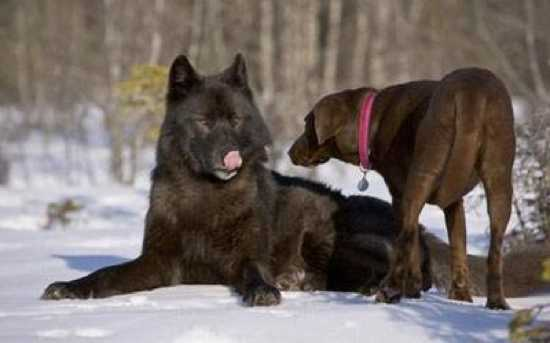
\includegraphics[scale=0.6]{imgs/cachorroELobo.jpg}            
  \caption{Um cachorro é um lobo juntos. Os cachorros são apenas lobos com genes que os deixam mais doceis.}
  \label{fig:MostrandoOCruzamentoPorCorte}
\end{figure} 

Os algoritmos geneticos usam uma abordagem semelhante aos criadores de animais só aplicados a vetores de dados, estes vetores são chamados de cromossomos. Chromossomos tem genes, que são os elementos do vetor, este podem ser binarios, inteiros ou números reais. A imagem \ref{fig:ExemploDeVetores} ilustra estes três tipos.\\ \\
\begin{figure}[H]
  \center
  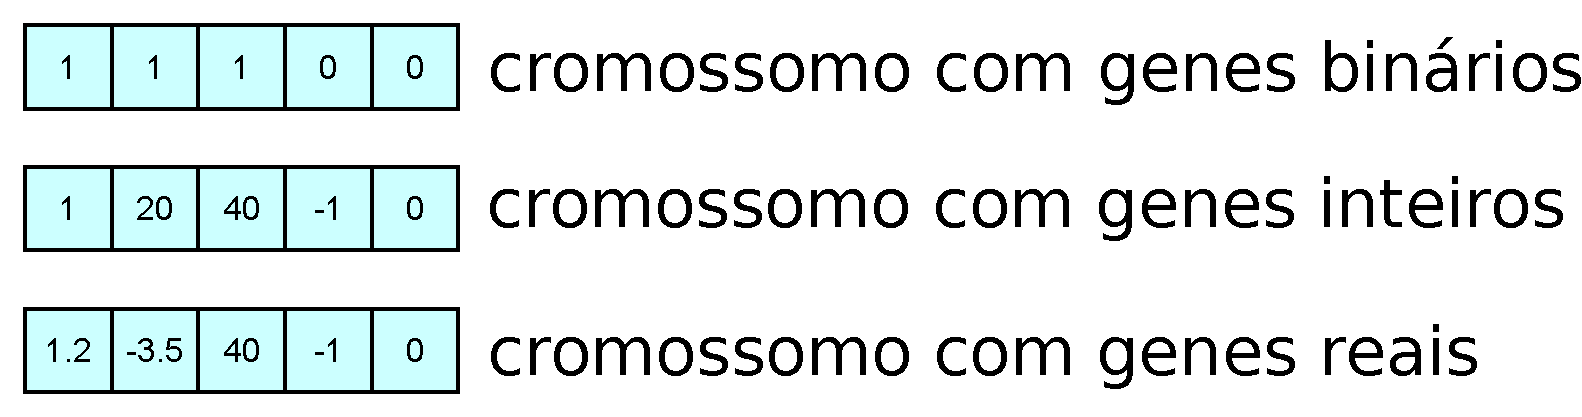
\includegraphics[scale=0.6]{imgs/tiposDeCromossomo.pdf}            
  \caption{Os varios tipos de genes que os cromossomos podem ter.}
  \label{fig:ExemploDeVetores}
\end{figure} 

A decisão sobre quais chromossomos são melhores para transmitir seus dados para as gerações futuras, o cruzamento, pertence a função a ser otimizada, chamada de função objetivo. A função objetivo apenas da uma pontuação a um chromossomo que diz o quão bom ele é para a função, quem decide se o chromossomo vai ou não passar suas caracteristica é o metodo de seleção. Existem dois metodos de seleção o da roleta, descrito em \cite{UFRGS-Apostila-GA} e \cite{Livro-De-IA}, e do tornei, descrito em   \cite{Livro-De-IA} .\\ \\
 Na seleção por roleta, com $N$ chromossomos, com $1 \le i \le N$, com $\vec{p}$ sendo o vetor que guarda as pontuação que cada chromossomo da geração atual recebe da função objetivo e com com $\vec{c}_i$ sendo algum chromossomo da geração atual. A possibilidade  $\vec{c}_i$ ser escolhido em cada cruzamento é de $\left [100 \left ( \frac{p_{i}}{\sum \limits_{j=i}^{n} p_{j}}\right ) \right ]\%$. \\ \\
A seleção por tornei possui varias variantes, a utilizada neste trabalho consiste em selecionar aleatoriamente quatro chromossomos da população chamados de $\gamma_{1},\gamma_{2},\gamma_{3},\gamma_{4}$ seleciona-se então entre $\gamma_{1}$ e $\gamma_{2}$ aquele que tem a maior pontuação este chromossomo é chamado de $\gamma_{5}$, depois seleciona-se  entre $\gamma_{3}$ e $\gamma_{4}$ aquele que tem a maior pontuação este chromossomo é chamado de $\gamma_{6}$. O cruzamento então é realizado entre $\gamma_{5}$ e $\gamma_{6}$. \\ \\
Após a escolha para os vetores existe um cruzamento entre eles. Neste cruzamento dois ou mais chromossomos, dos escolhidos, se unem para criar novos chromossomos. O número de chromossomos criados por um cruzamento geralmente igual a quantidade de chromossomos que se juntataram para o cruzamento. Existem duas maneiras principais para se fazer o cruzamento a uniforme e a por corte. \\ \\
No cruzamento por corte genes de regiões estabelecidadas dos chromossomos pais, geração atual, vão para os chromossomos filhos, geração seguinte. A imagem \ref{fig:MostrandoOCruzamentoPorCorte} mostra o cruzamento por corte. \\ 
\begin{figure}[H]
  \center
  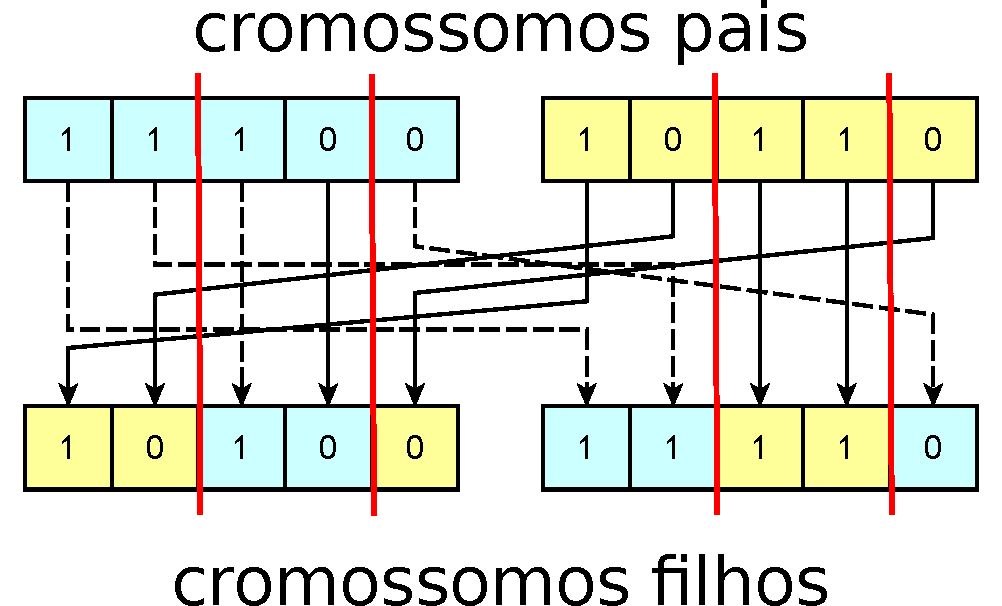
\includegraphics[scale=0.6]{imgs/diagramaCorte.pdf}            
  \caption{Cruzamento por corte entre dois cromossomos gerando dois novos Chromossomos. Neste cruzamento existe dois pontos de corte.}
  \label{fig:MostrandoOCruzamentoPorCorte}
\end{figure} 

No cruzamento uniforme cada vez que um grupo de chromossomos pais se unem para formar um filho é gerada uma mascara. Esta mascara diz que genes de um determinado chromossomos pai o filho vai receber. A imagem \ref{fig:MostrandoOCruzamentoUniforme} mostra o cruzamento uniforme. \\ \\
\begin{figure}[H]
  \center
  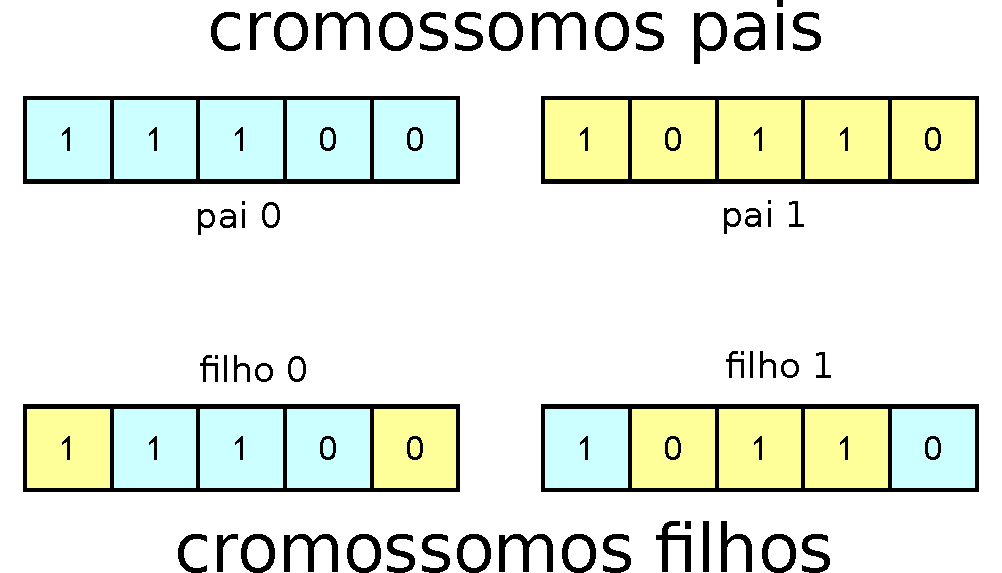
\includegraphics[scale=0.6]{imgs/diagramaMascara.pdf}            
  \caption{Cruzamento uniforme, através da mascara 10001.}
  \label{fig:MostrandoOCruzamentoUniforme}
\end{figure} \
Apos o cruzamento os cromossomos criados tem uma possibilidade de ter genes alterados aleatoriamente, isto é chamado de mutação. A mutação é importante para se sair do maximo de uma função objetivo. Porem ela não pode ser muito frequente por que uma mutação frequente faria com que os cromossomos criados fossem apenas vetores aleatorios.\\ \\
Assim os algoritmos geneticos podem ser definido pelo diagrama da imagem \ref{fig:DiagramaAG}. Este diagrama basicamente diz que se tem uma população inicial, geralmente gerada aleatoriamente, de chromossomos, chamada aqui de população $\alpha$. A partir deste ponto acontece uma repetição do processo. Os chromossomos são então submetidos a uma função objetivo ela diz o quão aptos eles são. Os Chromossomos são escolhidos para cruzamento com base na aptidão deles, isto gera uma nova população de chromossomos, chamada aqui de população $\beta$ .Alguns genes dos chromossomos da população $\beta$ são então alterados de maneira aleatoria, eles sofrem a mutação. A população $\beta$ se transforma-se na população $\alpha$. Repete-se o processo denovo então por $M$ vezes a partir do ponto de repetição estabelecido anteriormente.
\begin{figure}[H]
  \center
  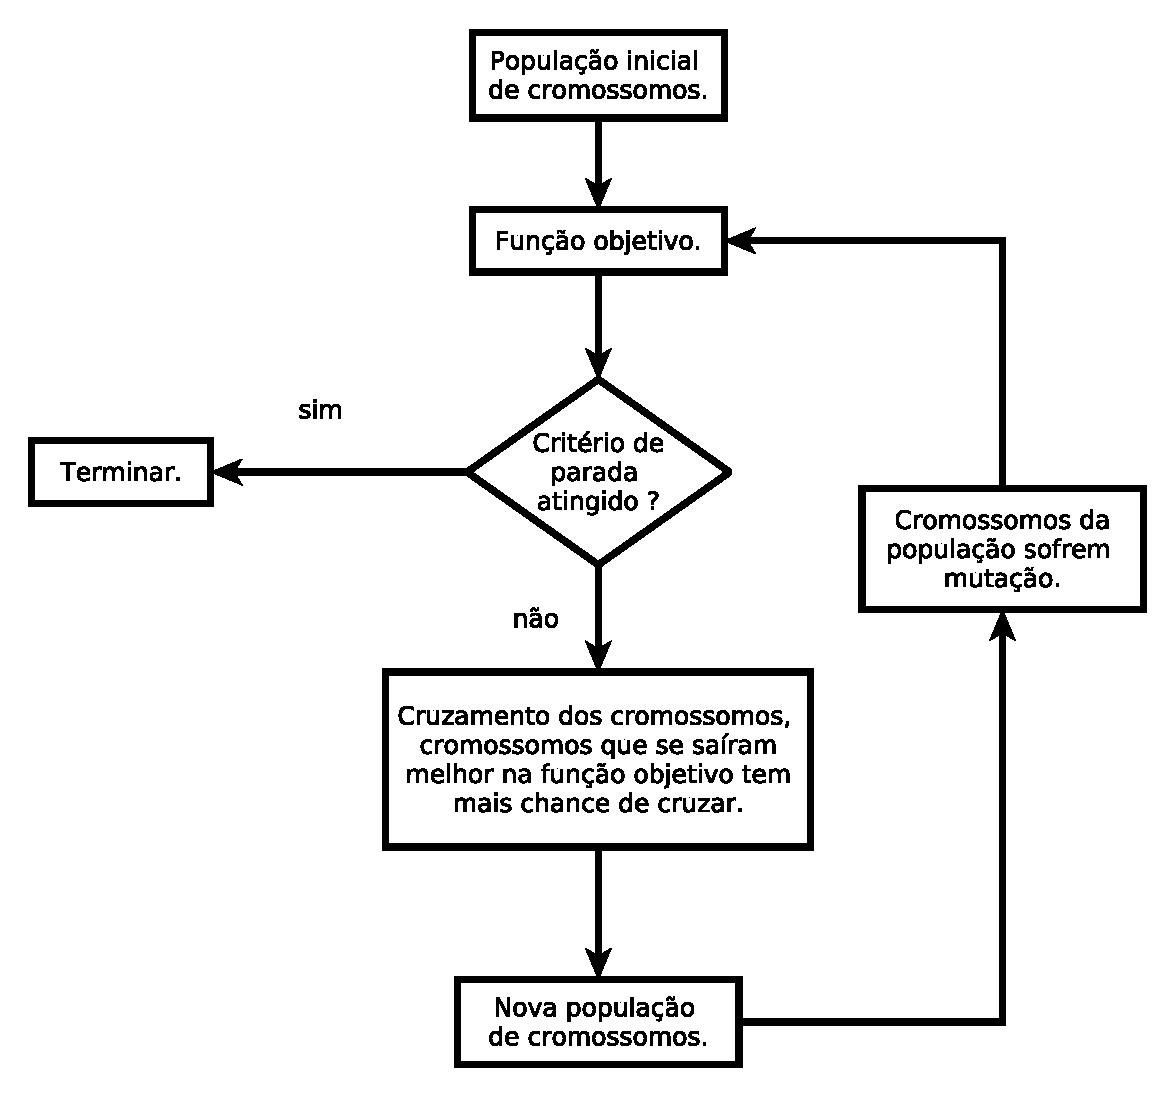
\includegraphics[scale=0.6]{imgs/diagramaAG.pdf}            
  \caption{Fluxograma ilustrando o conceito de algoritmos geneticos.}
  \label{fig:MostrandoOCruzamentoUniforme}
\end{figure}
\subsection{Angry Birds}
\label{sec:angryBirds}
O Angry Birds é um popular jogo de dispositivos portateis (celulares) e computadores, a imagem \ref{fig:AngryBirds} mostra um screenshot do jogo). O ojetivo do jogo é jogar passaros com um estilingue é acertar todos os porcos que estão no cenario com o menor número de passaros possivel, caso não seja possivel se acertar todos os porcos com o número de passaros que jogo fornece o player perde o jogo. A interação  e recepeção de dados do ambiente para o agente é efeita a partir screenshots tiradas do ambiente, o agente então usando algoritmos de visão computacional tem uma percepção completa sobre a situação do nível em que esta jogando.   \\ \\
O ambiente para o jogo possui pode ser descrito como: 
\begin{itemize}
\item Completamente observavel. Pois o framework permite, atravês do uso de vizão computacional, que o agente tenha um conhecimento sobre todas informações pertinentes ao ambiente para que ele tome suas escolhas. Entre as informações providas pelo framework estão: Saber onde estão os inimigos, saber quais são estruturas do ambiente que são interativas e a que classe elas pertencem, saber o tipo de munição ("passarinho") que o agente.
\item  Não determinístico. Pois jogadas iguais produzem pontuações diferentes, o video gravado \cite{videoMostrandoQueOjogoNaoEDeterministico} mostra isto. Isto acontece por que possivelmente a simulação fisica de colisão e gravidade usa metodos de monte carlo, uma vez que estes metodos de simulação são mais baratos computacionalmente. Porem não foi achado nenhum documento no site do Angry Birds dizendo isto.
\item Sequencial. Por que conforme se atira passaros nos porcos o ambiente vai mudando, por exemplo os blocos caindo, é o agente pode usar esta mudança a seu favor.
\item Estatico. Isto depende do agente, no caso da implementação realizada neste trabalho o agente espera o ambiente se estabilizar entre os arremessos de passaros. Por estabilizar se entende esperar que um novo passaro só vai ser jogado após os blocos e pedras do ambiente ja tiverem sé movido após o arremesso do passaro anterior, isto é feito esperando-se 15 segundos entre cada arremesso de passaro.  No entanto pode-se criar um agente que arremesse um passaro seguido do outro, com uma pausa entre a jogadas tão pequena que enquanto um passaro esta ainda esta atingindo algo no ambiente (oque vai mudar o ambiente) outro já foi arremessado. 
\item Continuo. Pois existem infinitos angulos e graus de força com que se pode arremessar os passros.
\item Agente único. 
\end{itemize}
\section{Modelagem do Angry Birds para algoritmos geneticos}
\label{sec:modelagem}
Para a modelagem se considerou que existem 3 tipos de genes, são eles:
\begin{itemize}
  \item Força,, que diz com que força um passaro é lançado do estilingue. Ele vai de  $0$ a $24$.
  \item Angulo,  que diz o angulo em que o passaro é arrmessado. Ele vai de  $0$ a $80$.
  \item Especial, que diz o tempo, em milesegundos, para ativação do especial a partir do momento em que o passaro é lançado do estilingue. Ele vai de  $0$ a $2500$.
\end{itemize}
O número de genes dos cromossomos depende da quantidade de passaros que o nível do jogo disponibiliza, pois cada passaro deve possuir uma força de arremesso, um angulo de arremesso e um tempo para ativação de seu especial (este gene pode ser desconsiderado para o passaro vermelho, por ele não possuir um especial). Para o nível 21, que foi o nivel em que foram realizados os testes deste trabalho, são 15 genes para cada cromossomo. Isso acontece porque este  nível possui 5 passaros amarelos. \\ \\
Para a função objetivo desta modelagem usa-se um determinado nível do jogo Angry Birds, o 21 neste caso. Assim se submete os cromossomos, de cada geração, a arremessar um grupo de 5 passaros (amarelos), depois dos arremessos cada cromossomo recebe do jogo uma nota por todos os seus arremessos. Como o objetivo deste trabalho é maximizar a função objetivo, ou seja obter a maior pontuação possivel em um nivel, os cromossomos que conseguem a maior pontuação são os mais aptos do ambiente. \\ \\
 Na modelagem deste trabalho, com o objetivo de tentar se preserva o maximo local, o melhor  cromossomo da geração atual sobrevive para a gereção seguinte. Outra caracteristica desta modelagem, para não ficar apenas no maximo local, é que a cada geração um cromossomo é gerado com genes aleatorios.
\section{Resultados}
Os dois principais resultados obtidos com este trabalho foram as taxas de apresendizagem, eficiencia, alcançada pelos metodos de seleção de cromossomos utilizados. Alem disto foi feita uma comparação do agente treinado, em ambos os metodos de seleção, com o agentes burro a partir do qual foram feito o agente deste trabalho. \\ \\
\subsection{Taxas de aprendizagem} 
Neste trabalho se consirou taxa de aprendizagem como sendo evolução da maximazação da função objetivo descrita na sessão \ref{sec:modelagem}. Deste modo a taxa de aprendizagem seria a evolução da pontuação maxima obtida pela população de cromossomos conforme as gerações passam, cromossomos estes que o agente utiliza para jogar Angry Birds em um determinado nível. \\ \\
Uma outra medida, complementar a taxa de aprendizagem, seria a evolução da média da pontuação obtida pela população de cromossomos, utilizados pelo agente, conforme se avança nas gerações. \\ \\
As figuras \ref{fig:taxaAprendizagemTorneio} e \ref{fig:taxaAprendizagem2Torneio} mostram o plot da taxa de aprendizagem e media de pontuação, para quando o agente é treinado com algoritmos geneticos que usam o metodo de seleção por torneio. A figura \ref{fig:taxaAprendizagemRoleta}  mostra o plot a taxa de aprendizagem e a figura \ref{fig:taxaAprendizagem2Roleta}  mostra o plot da media de pontuação, quando o agente é treinado com algoritmos geneticos que usam o metodo de seleção por torneio. \\ \\
\begin{figure}[H]
  \center
  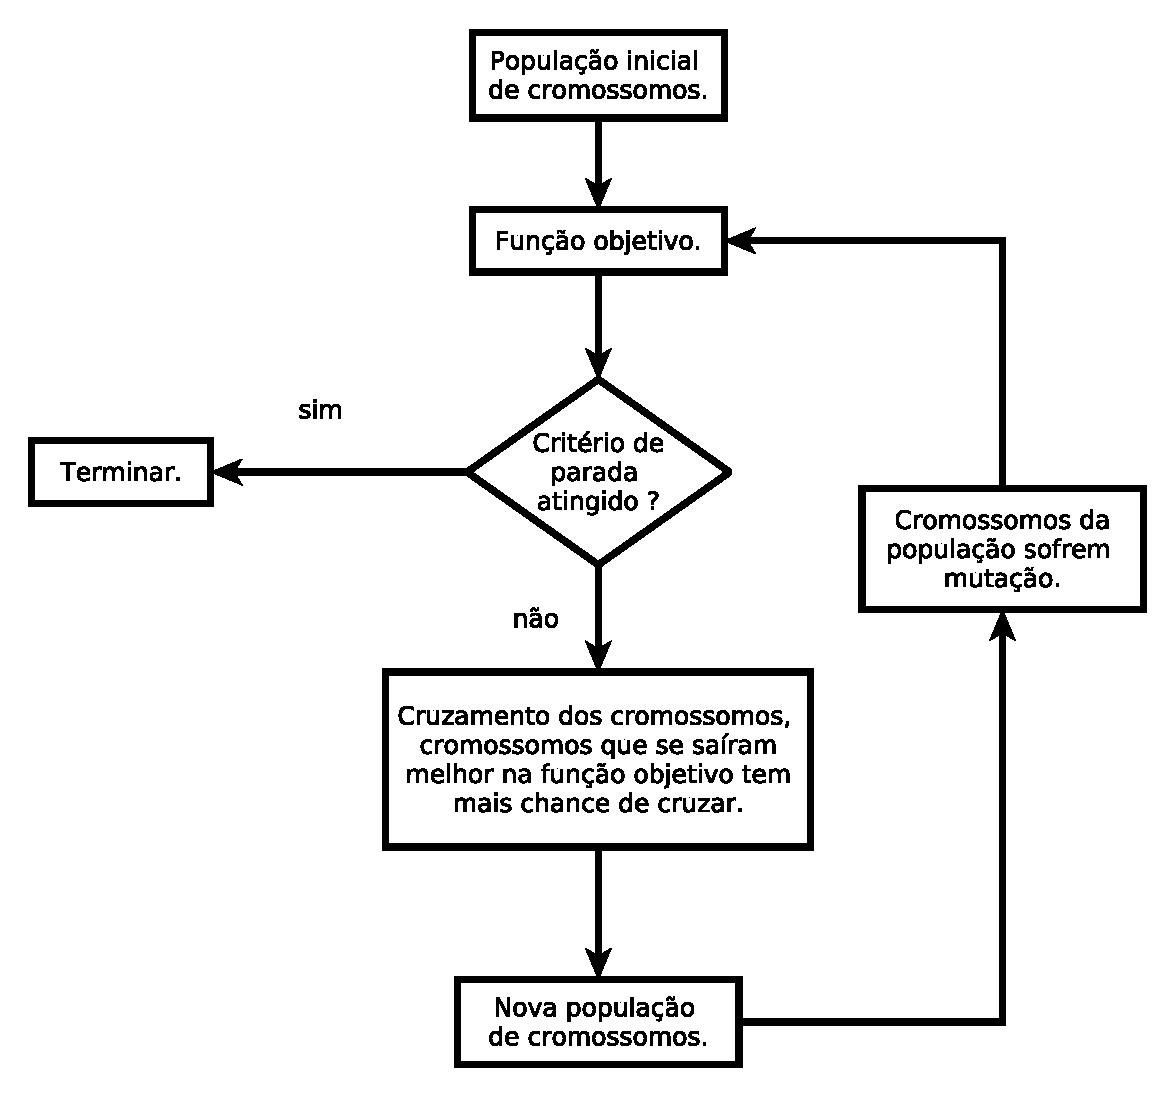
\includegraphics[scale=0.6]{imgs/diagramaAG.pdf}            
  \caption{Fluxograma ilustrando o conceito de algoritmos geneticos.}
  \label{fig:MostrandoOCruzamentoUniforme}
\end{figure}
\begin{figure}[H]
  \center
  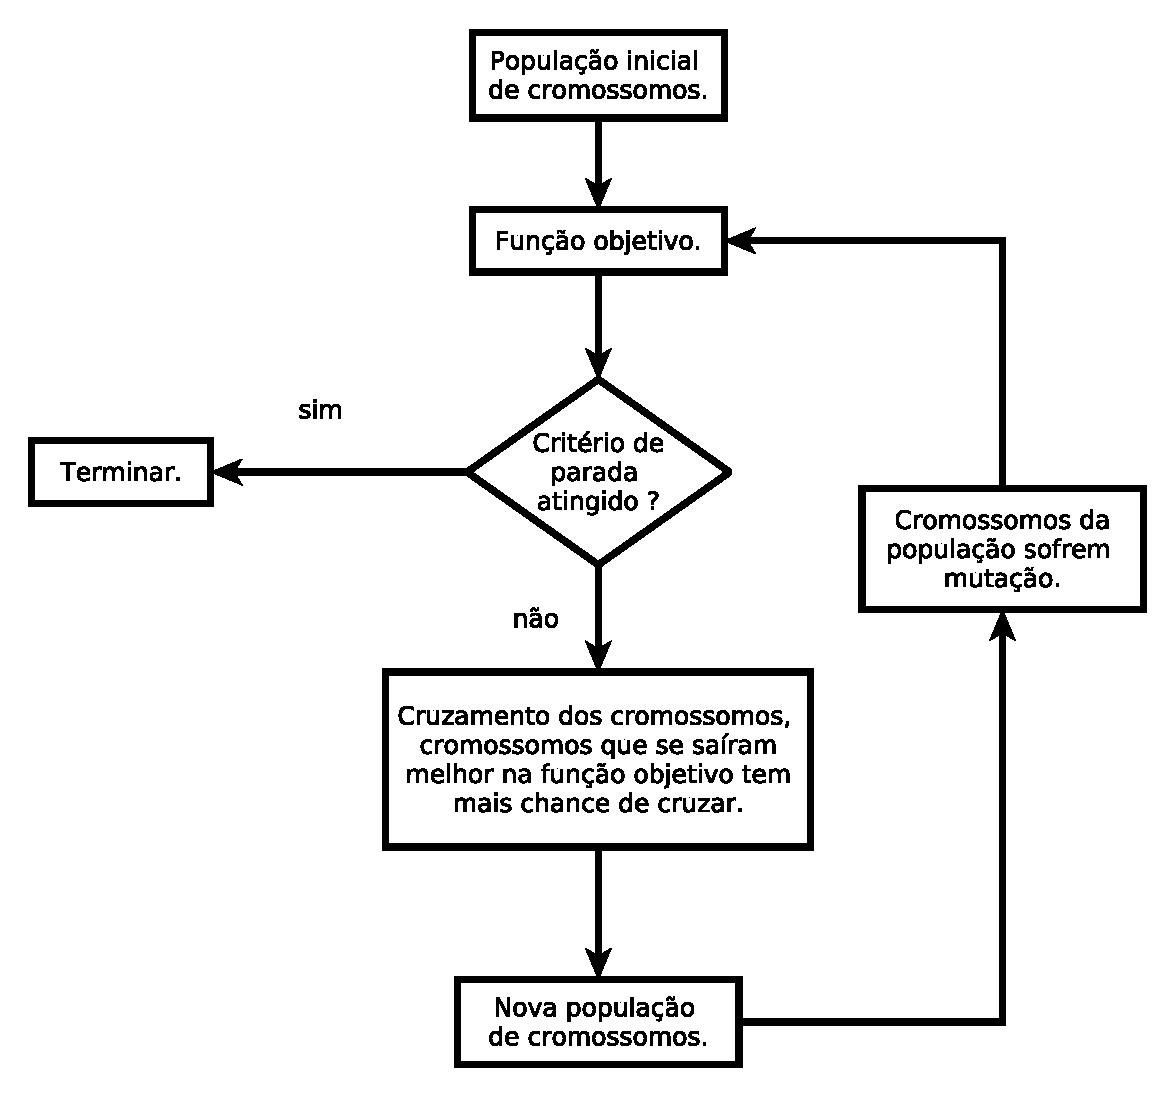
\includegraphics[scale=0.6]{imgs/diagramaAG.pdf}            
  \caption{Fluxograma ilustrando o conceito de algoritmos geneticos.}
  \label{fig:MostrandoOCruzamentoUniforme}
\end{figure}

Como pode-se ver o metodo da roleta, aprezentou uma taxa de aprendizagem maior que o metodo do torneio. Isto pode ser visto matematicamente, devirando-se a funções $g(x)$ e $h(x)$  para as quais a taxa de aprendizagem de ambos os metodos foram ajustada. Uma vez que $g'(x)=$ e $h'(x)$ então $g()>h(x)$ pois $\lim_{n} \frac{g'(x)}{h'(x)}=0$ assim temos que a derivada para o metodo da roleta é $$ que é uma derivada  que cresce mais rapido que a derivada $ $ .\\ \\
Alem disto o metodo da roleta também aprensentou um melhor avanço na media de acertos da população de cromossomos, utilizados para jogar Angry Birds, conforme  se passam as gerações. A demonstração matematica disto é analoga a mostrada no paragrafo anterior, basta substituir $g(x)$ por $\gamma(x)$ e $h(x)$ por $\phi(x)$. \\ \\
 Assim o metodo da roleta é melhor, do que o metodo  por torneio, em um ambiente de aprendizado como o descrito na seção \ref{sec:angryBirds}.
\subsection{Comparação entre agentes treinados com o agente burro}
Para esta comparação foi adotado o criterio de se pegar o melhor cromossomo gerado pelo metodo da roleta, o melhor cromossomo gerado pelo metodo do torneio e comparar a pontuação que eles obtem junto com a pontuação que o agente burro obtem. \\ 
Para obter-se a pontuação a partir do agente burro se jogou o nivel 20 com ele 10 vezes, a partir disso foi extraido uma media e um desvio padrão da pontuação das jogdas no Angry Birds. Além disto também sera mostrado a pontuação maxima e minima que o agente burro conseguiu no jogo. \\ \\ 
Para os cromossomos utilizou-se também o criterio de o agente jogar com cada cromossomo 10 vezes, para poder se extrair uma media e desvio padrão pontuação que cada um dois cromossomos consegue. Isto foi feito por que conforme dito na seção \ref{sec:angryBirds} o ambiente em que os agentes foram treinados possui um certo grau não determinismo. \\ \\
A tabela \ref{tab:comparacao} apresenta as medidas, desvios padrões, pontuação maxima e pontuação minima que os dos cromossomo selecionados junto com o agente burro obtiveram.
\begin{table}[h]
  \small
  \begin{tabular}{|L{5cm}|l|l|l|l|}%
    \hline                                                                    
    \textbf{} & \textbf{Média} & \textbf{Desvio Padrão} & \textbf{Maxímo} & \textbf{Mínimo} \\ \hline 
    Agente burro & 17341 & 2688.633 & 21390 & 13720 \\ \hline
    Agente criado  pelo cromossomo obtido pelo método da roleta & 7 & 31049 & 9236.183 & 47270 & 12240 \\ \hline
    Agente criado pelo cromossomo obtido pelo método do torneio & 28229 & 8720.646 & 49670  & 19950 \\ \hline
  \end{tabular}
  \caption{Média, desvio Padrão, maxímo e mínimo da pontuação que o agente burro e os agentes criados pelos cromossomos, obtidos pelos metodos roleta e torneio, conseguem no Jogo Angry Birds. Estes dados foram obtidos a partir de 10 partidas realizadas por cada um dos agentes criados.}
  \label{tab:comparacaoDosAgentes}    
\end{table}
\section{Conclusão}
Neste trabalho foi feita uma comparação entre dois metodos para seleção de cromossomo em algoritmos geneticos. Usando-se como base para comparação o ambiente do jogo Angry Birds.  As analises mostram que o metodo de seleção por roleta se saiu melhor para o ambiente do jogo. \\ \\
Também foi realizada uma comparação de pontuação entre os agentes criados pelos melhores cromossomos obtidos por ambos os metodos de seleção, de algoritmos geneticos, com um agente burro disponibilizado pelo site IA-Birds. Ambos os agentes criados apartir dos cromossomos foram melhor que o agente burro. Oque mostra que algoritmos geneticos é um bom metodo de IA para resolução de problemas como descritos pelo ambiente do Angry Birds.
\bibliography{bibliografia}
\bibliographystyle{plain}
\end{document}

\message{ !name(sumarioExecutivo.tex) !offset(-151) }
